\documentclass[../mattg_ti-fi_lit-review.tex]{subfiles}

There has been much interest in creating spintronic devices for modern applications. One focus in particular is a heterostructure (two or more layers) that creates a spin-torque device. That is, some ferromagnetic layer that is switchable by running an electric current through another layer. Researchers have been trying to make these devices a reality using a heterostructure of a topological insulator and ferromagnetic materials for about 10 years, since the first suggestions \cite{moore_birth_2010, garate_inverse_2010} of such applications of TIs.

Here I will outline the basic mechanics (what makes the wheels spin) of a spin-torque device, as well as the measurements and figures of merit by which to judge their success. I will show some significant results for conductive and insulating ferromagnetic materials, and identify gaps in experiments.

\subsection{Spin Torque Devices}

There have been some theoretical predictions for spin-torque devices for a while, considering metallic ferromagnet - topological insulator heterostructures as spin torque devices \cite{garate_inverse_2010, ghosh_spin-orbit_2018}, the likes of which we want to fabricate.

This idea is not new with the introduction of TI materials, rather it has been established in ferromagnetic multilayers. In 1996 Slonczewski predicted the generation of a spin current through the use of a fixed initial ferromagnetic material, before channelling that current into a secondary ferromagnetic material consequently applying a torque \cite{slonczewski_current-driven_1996}. The initial material remains ferromagnetically fixed due to two possible reasons. A initial material thicker than the secondary layer can be less susceptible to spin-transfer torque. Another possibility is exchange biasing by coupling to an antiferromagnet.

A recent review article by Locatelli, Cros and Grollier \cite{locatelli_spin-torque_2014} describes the achievements thus far in typical spin torque devices primarily coming through devices that have magnetoresistive readout of magnetic states and small cross-sectional area. The resistance is proportional to the magnetic state, typically through a "giant magnetoresistance effect" (GMR). 

More recently heavy metal and ferromagnetic heterostructures have led to observing spin-torque through large spin orbit coupling. 




The basic mechanism is that a current that runs through the surface state of a topological insulator is momentum-spin locked - this means there's a net spin polarisation for carriers moving in a particular direction. The idea is that this spin density is strong enough to influence the ferromagnetic material that is within proximity. 




This scenario is shown in Fig. \ref{fig:hetero-schematic}, from Li \etal{}, in which small metallic ferromagnetic pads produced $\mu$V responses to mA currents \cite{li_electrical_2014}.

\begin{figure}
	\centering
	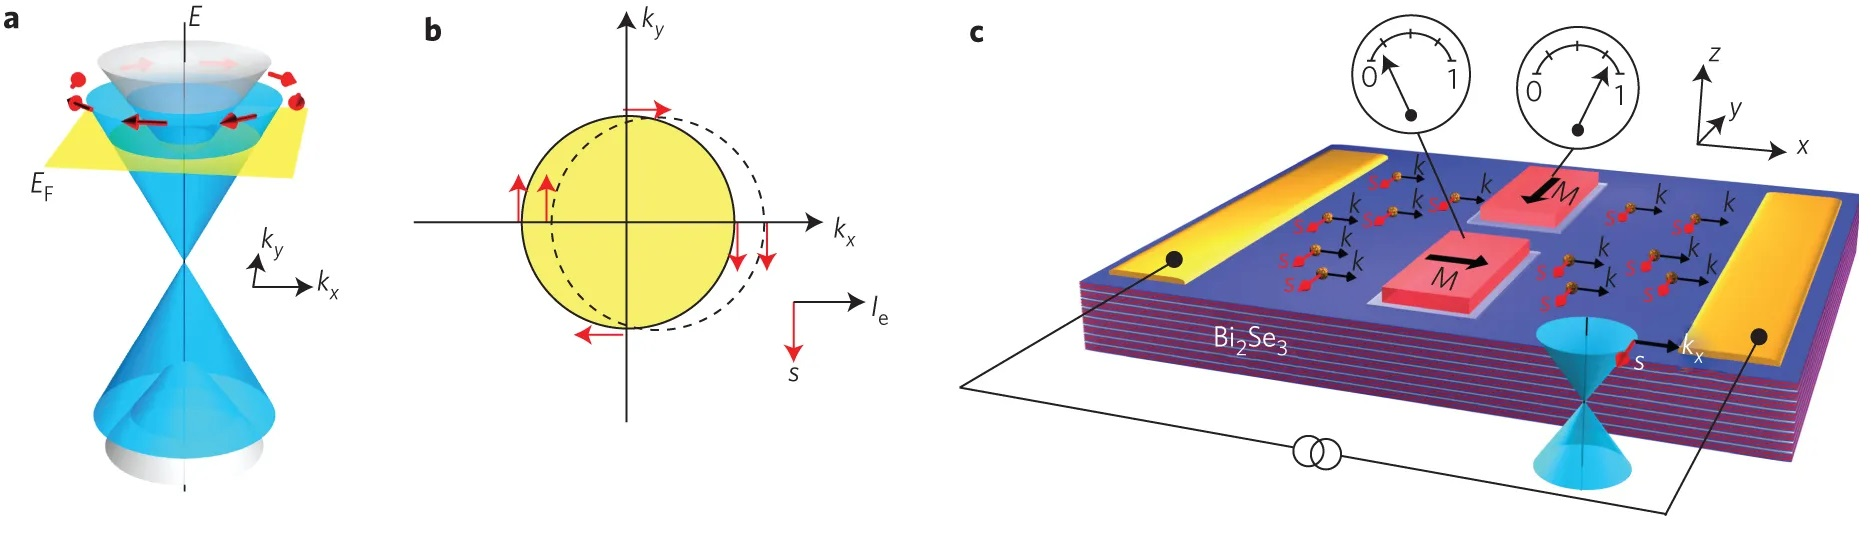
\includegraphics[width=\textwidth]{hetero-schematic}
	\caption{\textbf{a)} Momentum-spin locking - a Dirac cone with spin pointing at right angles to momentum. \textbf{b)} Top view of a slice of $k_x$-$k_y$ plane. An applied voltage produces a net momentum, and a net spin-current. \textbf{c)} The transport system, where spin polarised currents drive transitions in local ferromagnets.\\
	Source: Li \etal{}\cite{li_electrical_2014}, Nature Nano. 9, 218 (2014)}
	\label{fig:hetero-schematic}
\end{figure}

In addition to the above effects, the proximity effect of the ferromagnetic material's field to topological insulator surface state can be used to break the time-reversal symmetry that protects the surface state, possibly acting as a transistor switch.

%TODO Proximity effect in detail?
%\subsection{Proximity Effect}
\subsubsection{Torque}
Total angular moment L. 
\begin{align}
\frac{d\vec{L}}{dt}=\vec{T}
\end{align}
A spin orbit torque (SOT) is described as
\begin{align}
\tau_{SO} &= -\gamma \textbf{M} \times \textbf{B}_{SO}
\end{align}
where $\gamma$ is gyromagnetic ratio for some effective $B_{SO}$.
%TODO Fill in details later with experiments.
%\subsubsection{Spin Torque Angle - Spin Torque Efficiency}
%\subsubsection{Magnetization}
%Larmor Equation:
%\begin{align}
%\vec{T} = \mu_0 \vec{\textbf{M}}\times \vec{\textbf{H}}
%\end{align}
%Gyromagnetic Ratio
%\begin{align}
%\gamma\equiv\frac{\mu}{L}
%\end{align}
%Magnetization Change
%\begin{align}
%\frac{d\vec{M}}{dt} = \gamma\vec{T}
%\end{align}
%\subsubsection{Critical Current Density}
%\subsubsection{Charge Spin Conversion Efficiency}

\subsection{Quantum Anomalous Hall Effect (QAHE)}\label{sec:QAHE}
The anomalous hall effect been observed in ferromagnetic materials for a long time. It's anomalous because it appears without the need of an external magnetic field. The origins for the effect can be both intrinsic, or extrinsic (system dependent disorder). 

It turns out that just like the Hall effect and the spin Hall effect have quantised versions, there also exists a quantum anomalous Hall effect (QAHE). The first observation of this was made by Chang \etal{} \cite{chang_experimental_2013} in the material Cr$_{0.15}$(Bi$_{0.1}$Sb$_0.9$)$_{1.85}$Te$_3$, shown in Fig. \ref{fig:hetero-qahe}. The signature of the QAHE is that the zero-field Hall resistance still exhibits a distinct plateau with the quantized value $h/e^2$ around $V_g=-1.5$ in sub-figure B. 
The particular sample used has a Curie temperature of $\sim15$ K, and a mobility of 760 \mobilityunits.

\begin{figure}
	\centering
	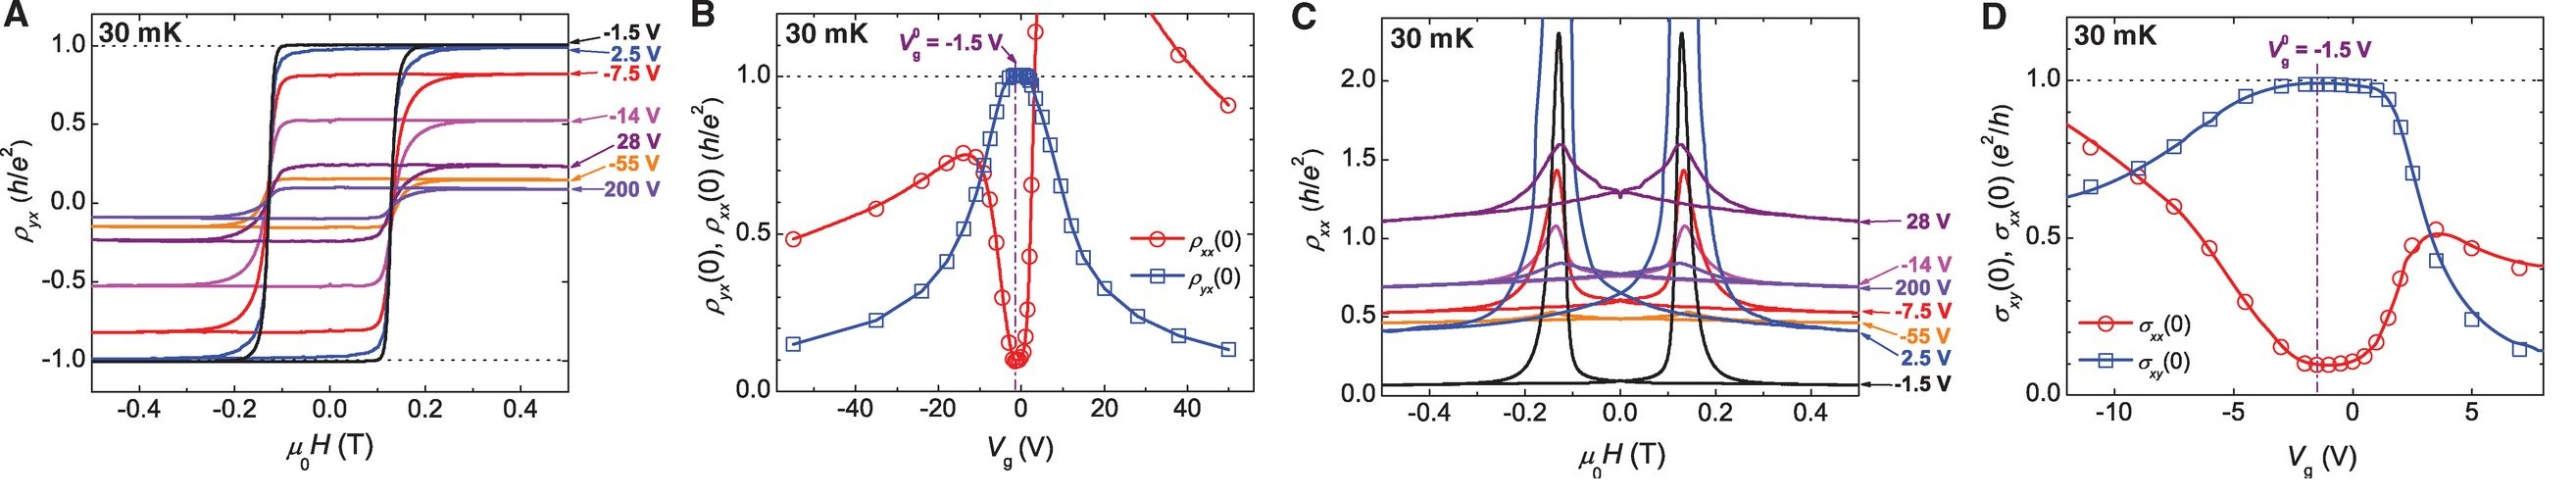
\includegraphics[width=\textwidth]{hetero-qahe}
	\caption{\textbf{a)} Magnetic field dependence of $\rho_{xy}$ for different $V_g$  
		\textbf{b)} Dependence of $\rho_{xy}$ (blue) and $\rho_{xx}$ (red) on $V_g$
		\textbf{c)} Magnetic field dependence of $\rho_{xx}$ for different $V_g$
		\textbf{d)} Dependence of $\sigma_{xy}$ (blue) and $\sigma_{xx}$ (red) on $V_g$\\
		Source: Chang \etal{}\cite{chang_experimental_2013}, Science Vol. 340, 167 (2013)}
	\label{fig:hetero-qahe}
\end{figure}

\subsection{Experiments}

\subsubsection{Conductive ferromagnetic films}
Mellnik \etal{} demonstrated the use of \bismuthselinide{} in conjunction with the ferroic permalloy Ni$_{81}$Fe$_19$. They also reported

\begin{itemize}
	\item $\sigma_{S,\parallel}$ = 2.0$\pm$0.4 $\times 10^5\hbar/2e$ $\Omega^{-1}$m$^{-1}$
	\item $\sigma_{S,\perp}$ = 1.6 $\pm$ 0.2
\end{itemize}

\begin{figure}
	\centering
	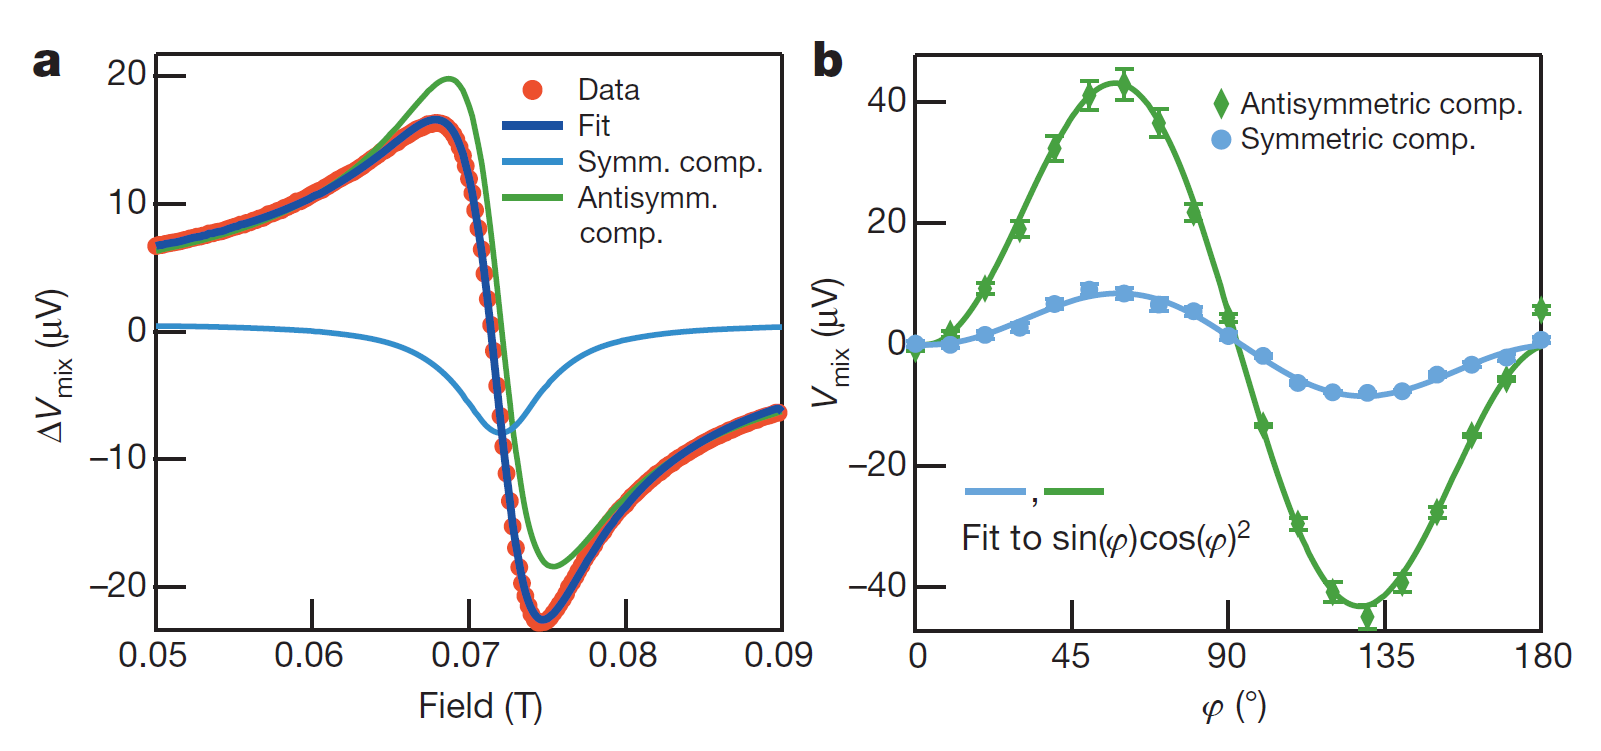
\includegraphics[width=\textwidth]{hetero-bi2se3-nife}
	\caption{\textbf{a)} Spin Torque Ferromagnetic Resonance of current induced torque, with fits. \textbf{b)} Dependence on magnetic field angle $\phi$.\\
		Source: Mellnik \etal{}\cite{mellnik_spin-transfer_2014}, Nature Vol. 511, 449 (2014)}
	\label{fig:hetero-bi2se3-nife}
\end{figure}

More recently, Wang \etal{} reported a spin-conversion efficiency of 1-1.75 in thin \bismuthselinide{} / NiFe heterostructures, with a switching current of $6\times 10^{5}$ A cm$^{-2}$ \cite{wang_room_2017}. This is roughly an order of magnitude smaller than with heavy metals.


\subsubsection{Insulating ferromagnetic films}

Wang \etal{} \cite{wang_surface-state-dominated_2016} used \bismuthselinide{} and (Bi,Sb)$_2$Te$_3$ on top a substrate of the ferromagnetic insulator film Y$_3$Fe$_5$O$_{12}$. The study conducts a TI thickness dependent examination of the spin-charge conversion efficiency, observing that it saturates at a maximum above a thickness of 6 quintuple layers.\\

\newcommand{\bisbtese}[4]{Bi$_{#1}$Sb$_{#1}$Te$_{#1}$Se$_{#1}$}
More recently, Chong \etal{} \cite{chong_topological_2018} creates GCGT / hBN and TI \bisbtese{2-x}{x}{3-y}{y} heterostructures, using graphite as a top gate (Fig. \ref{fig:hetero-bsts-gct}). This is a detailed transport study, but they do not see the emergence of the QAHE at zero magnetic field, and measure very little asymmetry between top and bottom gate behaviour. They do observe a maximum quantised Hall resistance of $h/e^2$ for a hBN device, however fail to show much significant magnetic field dependent behaviour for their CGT heterostructures. They suggest that they've opened a bandgap, this is not very convincing. Note that the supplementary material offers a lot more information into their 3 CGT devices. 

\begin{figure}[]
	\centering
	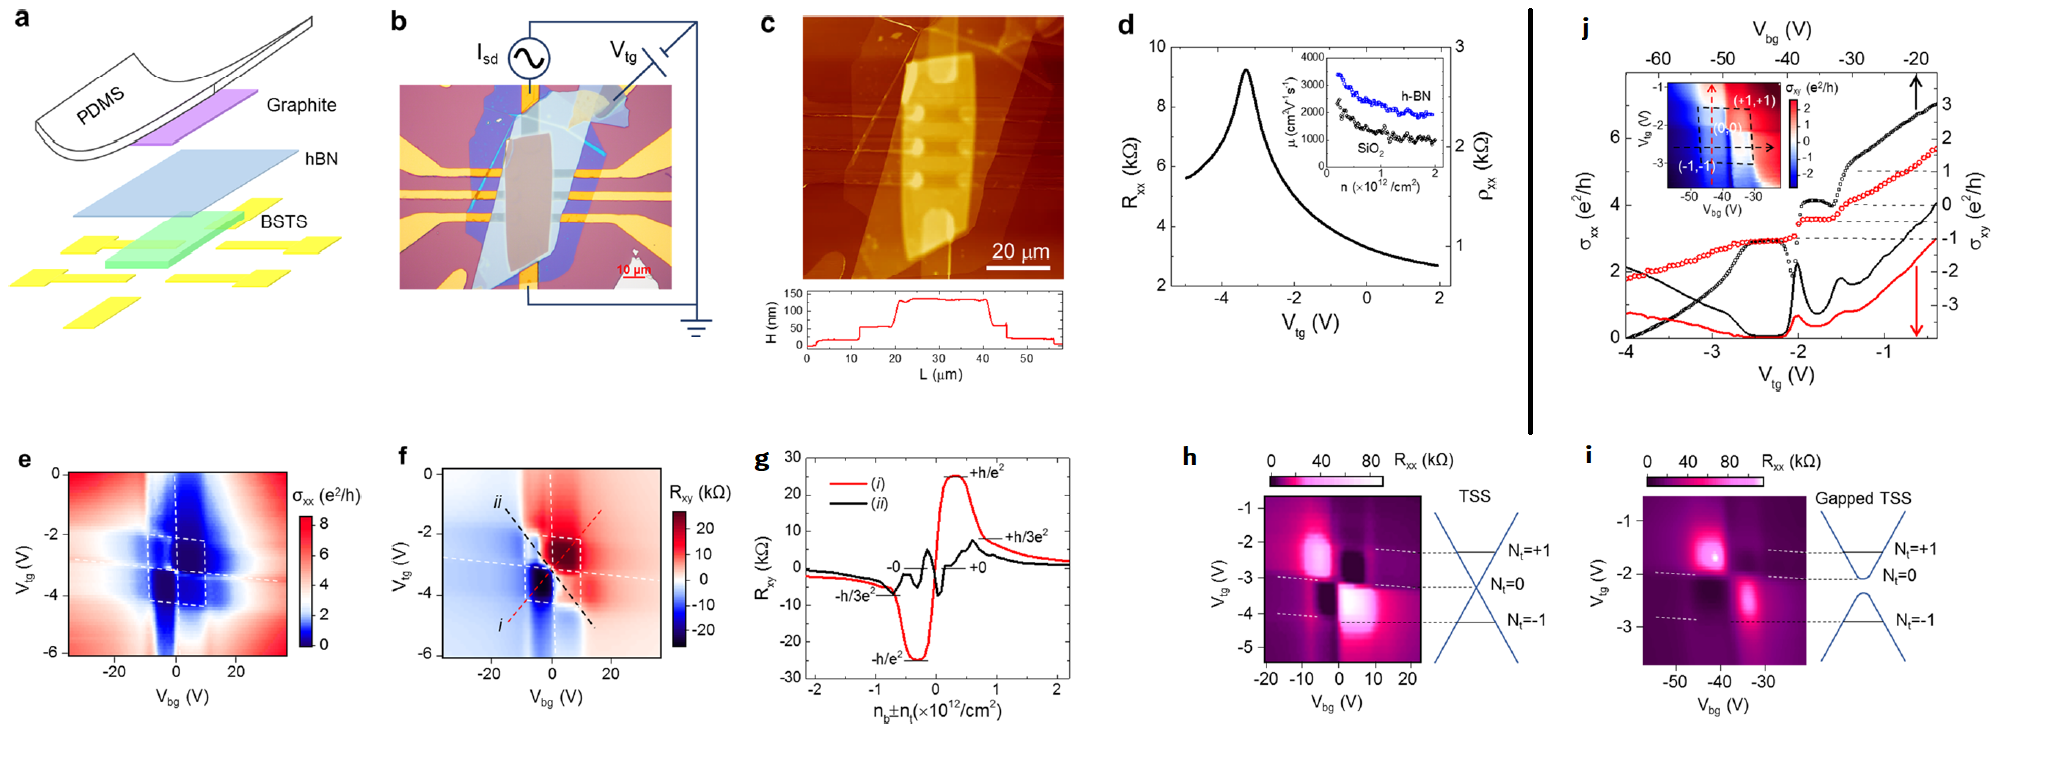
\includegraphics[width=\textwidth]{hetero-bsts-cgt}
	\caption{\textbf{a-h) hBN device a)} Schematic \textbf{b)} Optical image \textbf{c)} AFM \textbf{d)} Gated resistance at 0T, 1.6K. \textbf{e-j) Transport at 9T} \textbf{e)} Longitudinal conductivity \textbf{f)} Hall resistance \textbf{g)} Line profiles of f) \textbf{h)} Ungapped topological surface state \textbf{i-j) CGT device i)} Gapped topological surface state \textbf{j)} Line profiles of inset\\
		Source: Chong \etal{}\cite{chong_topological_2018}, Nano Lett. 18, 8047 (2018)}
	\label{fig:hetero-bsts-gct}
\end{figure}

\subsubsection{Not-quite TI-Ferromagnetic heterostructures}
In 2014, Fan \etal{}\cite{fan_magnetization_2014} reported the observation of magnetised switching in a chromium-doped (Bi$_{0.5}$Sb$_0.5$)$_2$Te$_3$ bilayer heterostructure at a critical current density of $8.9 \times 10^4$ A cm$^{-2}$ at 1.9 K. However, this system is not only 3D spin-hall effects, but also Rashba interfacial interactions, and so the torque is not directly understood in terms of the topological surface state. The switching of the AHE resistance is shown in Fig. \ref{fig:hetero-bisbte}.

\begin{figure}
	\centering
	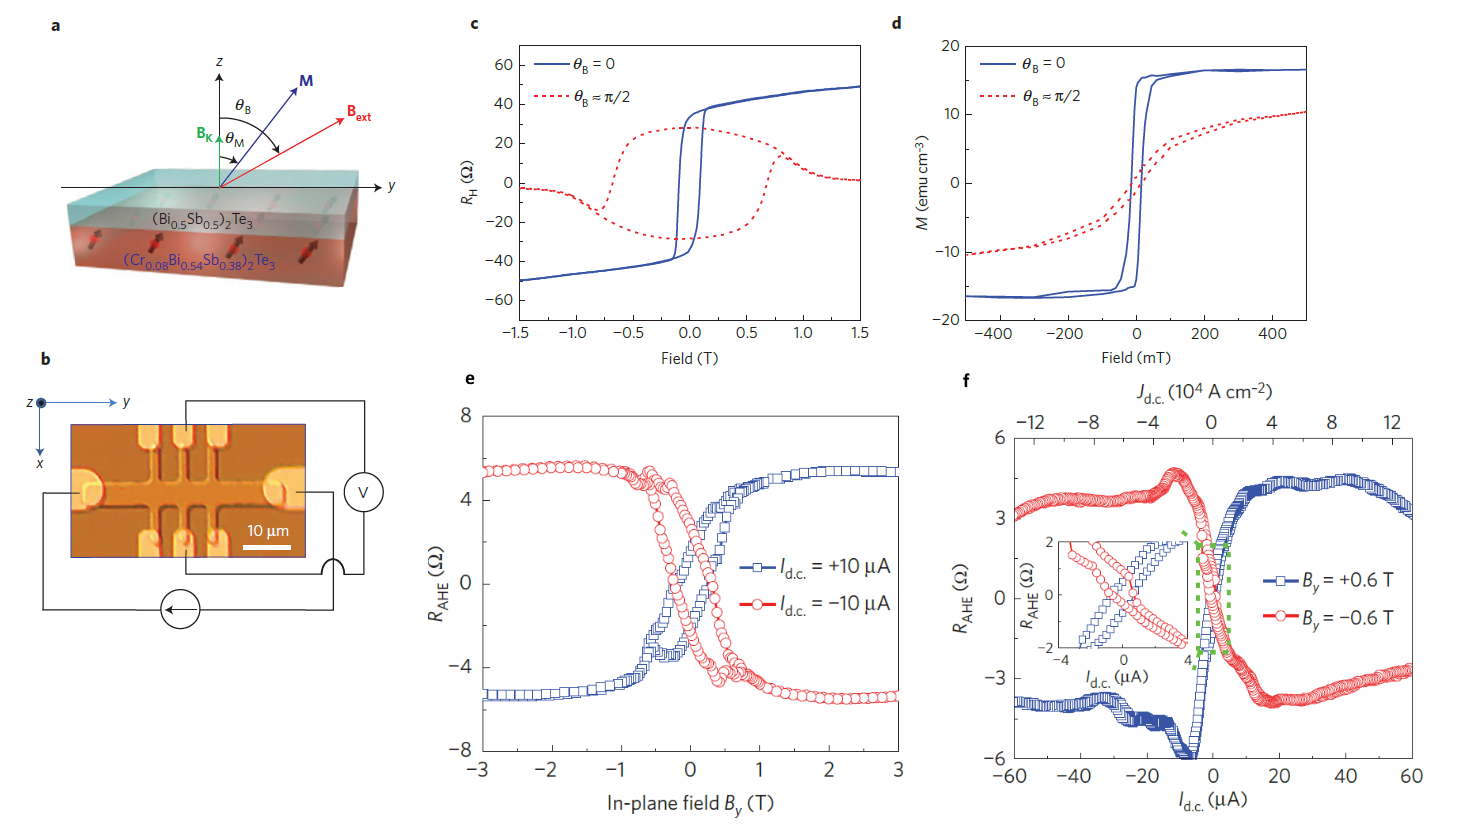
\includegraphics[width=0.8\textwidth]{hetero-bisbte}
	\caption{\textbf{a)} Bilayer heterostructure. Top (blue) 3 quintuple layers, bottom (red) 6 quintuple layers. \textbf{b)} Microscopy \textbf{c,d)} Hall resistance and magnetisation of sample. \textbf{e,f)} Current induced and field induced AH resistance.\\
	Source: Fan \etal{}\cite{fan_magnetization_2014}, Nature Mat. Vol. 13, 699 (2014)}
	\label{fig:hetero-bisbte}
\end{figure}

%\textcolor{red}{TODO: go through past experiments. Take significant of results, sample fabrication, experimental methodology}.
%\subsubsection{Conductive films (non-insulating)}
%\begin{itemize}[noitemsep,topsep=0pt,parsep=0pt,partopsep=0pt]
%	\item (2012) Liu et al. Beta-Ta with CoFeB  (Observed Torque, 2.1mT for 0.7mA, Sputtered/evaporated onto surfaces) 
%	\item (Apr 2013) Chang et al. Observation of QAHE - Cr0.15(Bi0.1Sb0.9)1.85Te3  - 5 quintuple layers, on SrTiO3, grown through MBE. Mobilities lower than 1000cm2/Vs. Chromium doping to make ferromagnetic, RHEED, ARPES.
%	\item (Apr 2014) Y. Fan et al. Epitaxial (Bi0.5Sb0.5)2Te3/(Cr0.08Bi0.54Sb0.38)2Te3 bilayer films, 3 \& 6 Quintuple layers respectively. AHE. ($\theta$SH reported to be very large??). Look again at device fab. 
%	\item (2014) A.R. Mellnik et al.  8nm Bi2Se3 and 8nm / 16nm Ni81Fe19 Bilayer (MBE \& Sputtering) (Observed Torque Applied, Torque per unit moment Tparallel = 2.7 x 10-5, T¬perp=3.7 x 10-5), 
%	$\omega$SH\_parallel=(2.0 ± 0.4) × 105/2e $\omega$-1 m-1 and  $\sigma$SH\_perp  = (1.6 ± 0.2) × 105/2e $\omega$-1 m-1
%	\item  (2016) P. Li et al. Pt/BaFe12O19 – Torque observed, value not mentioned. 
% 	\item (Aug 2017) J. Han et al. (MIT \& Samarth Grp) - GaAs / Bi2Se3(7.4nm)/CoTb(4.6nm)/SiNx(3 nm) - Magnetron and MBE. Critical current density 2.8 x 106 A/cm$^2$. 
%	0.16 effective SH angle. Large discrepancies noted in this paper. Also searched (Bi, Sb)2Te3, and compared to Pt and other heavy metals.
%	\item (Sep 2017) K. Yasuda et al. Crx(Bi1-ySby)2-xTe3/(Bi1-ySby)2Te3 - Magnetic non-magnetic heterostructures. Second Harmonic Voltage goverened by asymmetric magnon scattering gives incorrect value of CSC (Charge spin conversion efficiency).
%	\item \textbf{(Nov 2017) Y. Wang et al. Bi2Se3/NiFe Heterostructure, Describes contamination of BS, 2DEG to the SOT effects from TSS affecting Bi2Se3 systems. Also used Bi2Se3/Co40Fe40B20, and Bi2Se3 (8 QL)/Py(6nm). Growths on Al2O3. Used MgO and Al2O3 to protect. Also SiO2 used for Py devices. Iron Milling used with Photolithography.}
%	\item (Jul 2018) Khang et al. Bi0.9Sb0.1, 5/10nm Mn0.45Ga0.55 3nm layers\\ $\sigma\approx2.5\times10^5\omega^{-1}m^{-1},\theta_{SH}\approx 52$ and $\theta_{SH}\approx1.3\times10^7\hbar / 2e \omega^{-1}m^{-1}$
%	\item (Jul 2018) Mahendra DC et al. BixSe(1-x)/Co20Fe60B20 (Magentron Sputtered)\\
%	$\theta_S = 18.62$ (d.c. planar Hall) \&8.67 (ST-FMR) [Si/SiO2/MgO (2nm)/BixSe(1-x)(tBS nm)/ CoFeB(5nm)/MgO(2nm)/Ta(5nm)] tBS=4,6,8,16,40nm
%	\item (Jan 2018) Y. Li et al.  Epitaxial (001) SmB6/Si thin films (50nm +) with MgO(1.5)/CFB(Co40Fe40B20, 1)/$\beta-W(0.8)$ – DC Magnetron sputtering / DC\&RF magnetron…
%\end{itemize}
%\subsubsection{Insulating Films}
%\begin{itemize}[noitemsep,topsep=0pt,parsep=0pt,partopsep=0pt]
%	\item (2019) P. Li et al. Bi2Se3 and FI - BaFe12O19 \url{https://advances.sciencemag.org/content/5/8/eaaw3415}
%	\item YIG (2016) H. Wang et al. \url{https://journals-aps-org.ezproxy.lib.monash.edu.au/prl/pdf/10.1103/PhysRevLett.117.076601}
%\end{itemize}
%
%\subsubsection{Non-TI Devices}
%- (2010) Co layer 0.6nm, with Pt 3nm and AlO\_x layers 2nm, transverse magnetic fields. https://www-nature-com.ezproxy.lib.monash.edu.au/articles/nmat2613?proof=trueMay

%TO READ:
%https://journals-aps-org.ezproxy.lib.monash.edu.au/prb/abstract/10.1103/PhysRevB.98.094404

